\documentclass[12pt]{article}

\usepackage{times}
\usepackage{graphicx}
\usepackage{mathtools}

\setlength{\textwidth}{6.5in}
\setlength{\textheight}{8.9in}
\setlength{\oddsidemargin}{0.0in}
\setlength{\topmargin}{0.05in}
\setlength{\headheight}{-0.05in}
\setlength{\headsep}{0.0in}

\begin{document}

\begin{center}
{\bf CS 6300} \hfill {\large\bf HW04: Value and Policy Iteration} \hfill {\bf Due Feb 21, 2023}
\end{center}

\section{Value Iteration}

In the MDP below, there are 5 states: C(ollege), G(rad school),
I(ndustry), A(cademia), and U(nemployed).  States I, A and U are
terminal states.  Probabilities of transitions are either 1/4 or 3/4,
and the values in parentheses are the rewards for that transition.
The possible actions from states C and G are:

      \begin{itemize}

      \item State C: You may choose to stay in C, but with a
        probability of 1/4 you may end up going to state G.

        You may also choose to go to state I, but with probability 1/4
        you end up in state U.

      \item State G: You may choose to stay in state G, but with
        probability 1/4 you end up in state U.

        You may also choose to go to state A, but with probability 3/4
        you end up in state I.

      \end{itemize}

  \begin{center}
  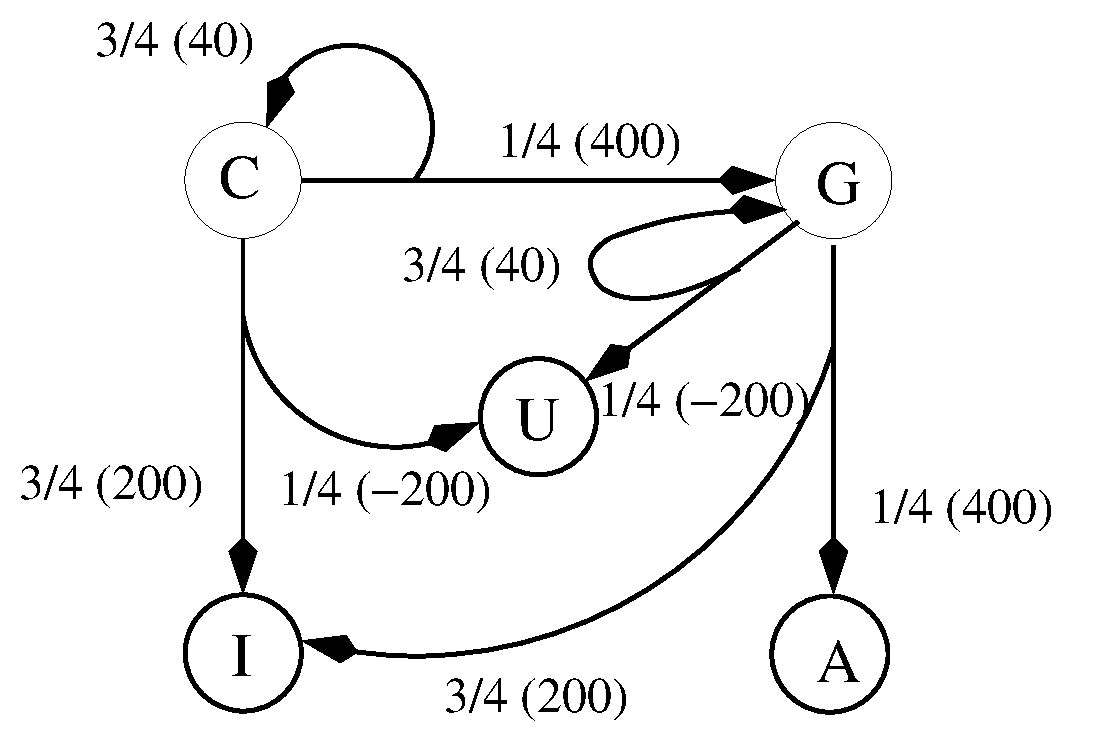
\includegraphics[height=2.5in]{cgiau.eps}
  \end{center}

\begin{enumerate}

\item You start in state C.  Perform two iterations of value
iteration, where you first compute the $Q$ values and then take
the maximum of the $Q$ values.  The discount is $\gamma = 1$.

\item Perform policy extraction after these two iterations to find $\pi^*(s)$.  Please show
    all work.

\end{enumerate}

\noindent
Round 1: \\
\noindent
$Q_1(C,C) = T(C,C,C)[(R(C,C,C)+V_0^*(C)]+T(C,C,G)[(R(C,C,G)+V_0^*(G)]$ \\
$Q_1(C,C) = \frac{3}{4} [40 + 0] + \frac{1}{4} [400 + 0] = 130$ \\

\noindent
$Q_1(C,I) = T(C,I,I)[(R(C,I,I)+V_0^*(I)]+T(C,I,U)[(R(C,I,U)+V_0^*(U)]$ \\
$Q_1(C,I) = \frac{3}{4} [200 + 0] + \frac{1}{4} [-200 + 0] = 100$ \\

\noindent
$Q_1(G,G) = T(G,G,G)[(R(G,G,G)+V_0^*(G)]+T(G,G,U)[(R(G,G,U)+V_0^*(U)]$ \\
$Q_1(G,G) = \frac{3}{4} [40 + 0] + \frac{1}{4} [-200 + 0] = -20$ \\

\noindent
$Q_1(G,A) = T(G,A,A)[(R(G,A,A)+V_0^*(A)]+T(G,A,I)[(R(G,A,I)+V_0^*(I)]$ \\
$Q_1(G,A) = \frac{1}{4} [400 + 0] + \frac{3}{4} [200 + 0] = 250$ \\

\noindent
Round 1 value update: \\
$V_1(C) = \max_{a \in \{C, I\}} Q_1^*(C,a) = 130$ \\
$V_1(G) = \max_{a \in \{G, A\}} Q_1^*(G,a) = 250$ \\ 
$V_1(I) = 0$ \\ 
$V_1(U) = 0$ \\ 
$V_1(A) = 0$ \\ 





\noindent
Round 2: \\
\noindent
$Q_1(C,C) = T(C,C,C)[(R(C,C,C)+V_1^*(C)]+T(C,C,G)[(R(C,C,G)+V_1^*(G)]$ \\
$Q_1(C,C) = \frac{3}{4} [40 + 130] + \frac{1}{4} [400 + 250] = 290$ \\

\noindent
$Q_1(C,I) = T(C,I,I)[(R(C,I,I)+V_1^*(I)]+T(C,I,U)[(R(C,I,U)+V_1^*(U)]$ \\
$Q_1(C,I) = \frac{3}{4} [200 + 0] + \frac{1}{4} [-200 + 0] = 100$ \\

\noindent
$Q_1(G,G) = T(G,G,G)[(R(G,G,G)+V_1^*(G)]+T(G,G,U)[(R(G,G,U)+V_1^*(U)]$ \\
$Q_1(G,G) = \frac{3}{4} [40 + 250] + \frac{1}{4} [-200 + 0] = 167.5$ \\

\noindent
$Q_1(G,A) = T(G,A,A)[(R(G,A,A)+V_1^*(A)]+T(G,A,I)[(R(G,A,I)+V_1^*(I)]$ \\
$Q_1(G,A) = \frac{1}{4} [400 + 0] + \frac{3}{4} [200 + 0] = 250$ \\

\noindent
Round 2 value update: \\
$V_2(C) = \max_{a \in \{C, I\}} Q_2^*(C,a) = 290$ \\
$V_2(G) = \max_{a \in \{G, A\}} Q_2^*(G,a) = 250$ \\ 
$V_2(I) = 0$ \\ 
$V_2(U) = 0$ \\ 
$V_2(A) = 0$ \\ 




\noindent
Policy extraction after 2 rounds: \\
$\pi_2(s) = arg \max_{a} \sum_{s'}T(s,a,s')[R(s,a,s') + V_i^*(s')]$


$\pi_2(C) =
  \begin{cases}
   T(C,C,C)[(R(C,C,C)+V_2^*(C)]+T(C,C,G)[(R(C,C,G)+V_2^*(G)] \\
   T(C,I,I)[(R(C,I,I)+V_2^*(I)]+T(C,I,U)[(R(C,I,U)+V_2^*(U)]
  \end{cases}
$ \\
$\pi_2(C) =
  \begin{cases}
    \frac{3}{4} [40 + 290] + \frac{1}{4} [400 + 250] = 410 \\
    \frac{3}{4} [200 + 0] + \frac{1}{4} [-200 + 0] = 100
  \end{cases}
$ \\
$\pi_2(C) = C$

$\pi_2(G) =
  \begin{cases}
   T(G,G,G)[(R(G,G,G)+V_2^*(G)]+T(G,G,U)[(R(G,G,U)+V_2^*(U)] \\
   T(G,A,A)[(R(G,A,A)+V_2^*(A)]+T(G,A,I)[(R(G,A,I)+V_2^*(I)]
  \end{cases}
$ \\
$\pi_2(G) =
  \begin{cases}
    \frac{3}{4} [40 + 250] + \frac{1}{4} [-200 + 0] = 167.5 \\
    \frac{1}{4} [400 + 0] + \frac{3}{4} [200 + 0] = 250
  \end{cases}
$ \\
$\pi_2(G) = A$


\clearpage

\section{Policy Iteration}

Consider again the following MDP.  There are 5 states: C(ollege),
G(rad school), I(ndustry), A(cademia), and U(nemployed).  States I, A
and U are terminal states.  Probabilities of transitions are either
1/4 or 3/4, and the values in parentheses are the rewards for that
transition.  The possible actions from states C and G are:

      \begin{itemize}

      \item State C: You may choose to stay $s$ in C, but with a
        probability of 1/4 you may end up going $g$ to state G.

        You may also choose to go $g$ to state I, but with probability 1/4
        you end up in state U.

      \item State G: You may choose to stay $s$ in state G, but with
        probability 1/4 you end up in state U.

        You may also choose to go $g$ to state A, but with probability 3/4
        you end up in state I.

      \end{itemize}

\noindent
You start in state C.  Assume your initial policy is $\pi_0(s) = s$,
i.e., you wish to stay in the current state you're in.  Also the
discount is $\gamma = 1$.

  \begin{center}
    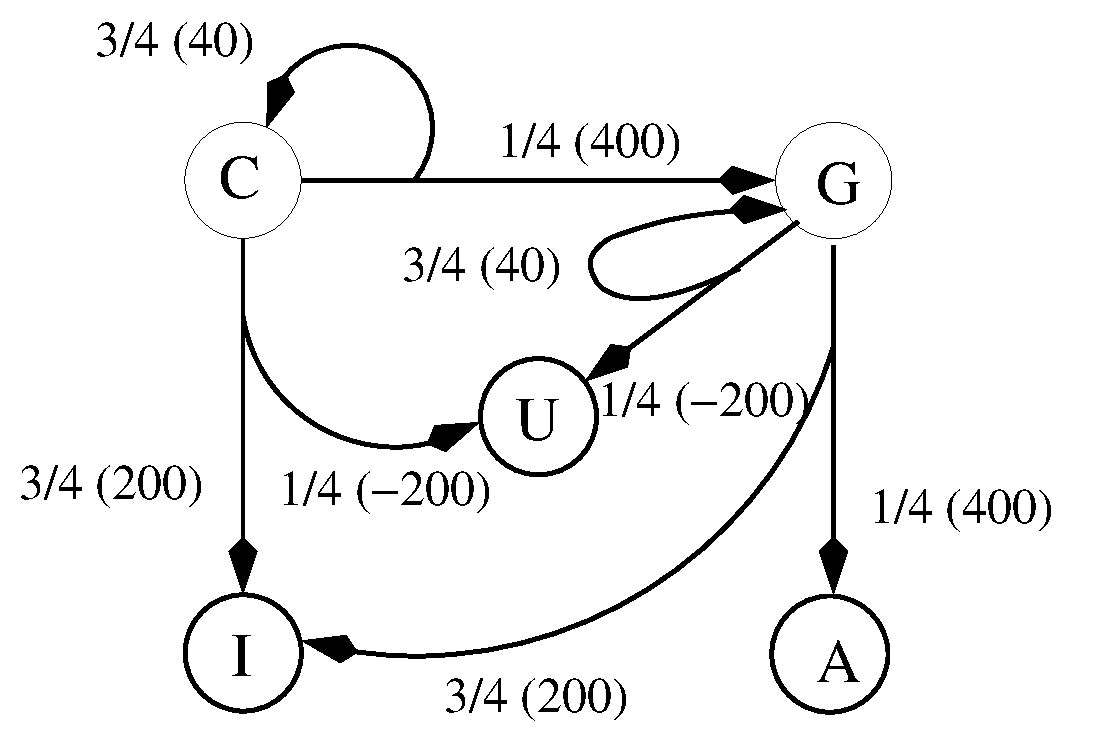
\includegraphics[height=2.5in]{cgiau.eps}
  \end{center}

For this problem you will perform one step of Policy Iteration:
  \begin{enumerate}

  \item Perform policy evaluation to solve for the utility values
    $V^{\pi_0}(C)$ and $V^{\pi_0}(G)$.  Remember that the
    utility values can be solved for analytically.

    The analytical equation to use is:
  $$V^{\pi_i}(s) = \sum_{s'} T(s,\pi(s),s') \left[ R(s,\pi(s),s') + \gamma  V^{\pi_i}(s') \right]$$

  \item Perform policy improvement to find $\pi_1(s)$.  Please show
    all work.

  \end{enumerate}

\noindent
$V^{\pi_0}(C) = \sum_{s'} T(C,\pi(C),s') [ R(C,\pi(C),s') + V^{\pi_0}(s')]$ \\
$V^{\pi_0}(C) = T(C,C,C)[(R(C,C,C)+V^{\pi_0}(C)]+T(C,C,G)[(R(C,C,G)+V^{\pi_0}(G)]$ \\
$V^{\pi_0}(C) = \frac{3}{4} [40 + 0] + \frac{1}{4} [400 + 0] = 130$

\noindent
$V^{\pi_0}(G) = \sum_{s'} T(G,\pi(G),s') [ R(C,\pi(G),s') + V^{\pi_0}(s')]$ \\
$V^{\pi_0}(G) = T(G,G,G)[(R(G,G,G)+V_0^{\pi_0}(G)]+T(G,G,U)[(R(G,G,U)+V_0^{\pi_0}(U)]$ \\
$V^{\pi_0}(G) = \frac{3}{4} [40 + 0] + \frac{1}{4} [-200 + 0] = -20$ \\

\noindent
Policy improvement: \\
$\pi_1(s) = arg \max_{a} \sum_{s'}T(s,a,s')[R(s,a,s') + V^{\pi_0}(s')]$


$\pi_2(C) =
  \begin{cases}
   T(C,C,C)[(R(C,C,C)+V^{\pi_0}(C)]+T(C,C,G)[(R(C,C,G)+V^{\pi_0}(G)] \\
   T(C,I,I)[(R(C,I,I)+V^{\pi_0}(I)]+T(C,I,U)[(R(C,I,U)+V^{\pi_0}(U)]
  \end{cases}
$ \\
$\pi_2(C) =
  \begin{cases}
    \frac{3}{4} [40 + 0] + \frac{1}{4} [400 + 0] = 130 \\
    \frac{3}{4} [200 + 0] + \frac{1}{4} [-200 + 0] = 100
  \end{cases}
$ \\
$\pi_2(C) = C$

$\pi_2(G) =
  \begin{cases}
   T(G,G,G)[(R(G,G,G)+V^{\pi_0}(G)]+T(G,G,U)[(R(G,G,U)+V^{\pi_0}(U)] \\
   T(G,A,A)[(R(G,A,A)+V^{\pi_0}(A)]+T(G,A,I)[(R(G,A,I)+V^{\pi_0}(I)]
  \end{cases}
$ \\
$\pi_2(G) =
  \begin{cases}
    \frac{3}{4} [40 + 0] + \frac{1}{4} [-200 + 0] = -20 \\
    \frac{1}{4} [400 + 0] + \frac{3}{4} [200 + 0] = 250
  \end{cases}
$ \\
$\pi_2(G) = A$

\end{document}